\documentclass[aspectratio=169,11pt,t]{beamer}

% ============================================================
% Theme and typography
% ============================================================
\usetheme{Madrid}
\usecolortheme{default}
\usefonttheme{professionalfonts}
\setbeamertemplate{navigation symbols}{}
\setbeamertemplate{headline}{}
\setbeamertemplate{footline}{%
  \leavevmode\hbox{%
  \begin{beamercolorbox}[wd=.82\paperwidth,ht=2.5ex,dp=1.0ex,leftskip=.8em]{author in head/foot}
    CSCI 2406 --- Computer Organization \& Architecture (AArch64 Reference)
  \end{beamercolorbox}%
  \begin{beamercolorbox}[wd=.18\paperwidth,ht=2.5ex,dp=1.0ex,rightskip=.8em]{date in head/foot}
    \hfill\insertframenumber/\inserttotalframenumber
  \end{beamercolorbox}}
}
\setbeamersize{text margin left=0.65cm,text margin right=0.65cm}
\setbeamerfont{frametitle}{size=\Large,series=\bfseries}
\setbeamerfont{block title}{size=\normalsize,series=\bfseries}
\setbeamertemplate{blocks}[rounded][shadow=false]
\addtobeamertemplate{block begin}{\vspace{0.05em}}{\vspace{0.05em}}
\addtobeamertemplate{block end}{}{\vspace{0.10em}}
\setbeamertemplate{itemize/enumerate body begin}{\setlength{\itemsep}{3pt}}
\setbeamertemplate{itemize/enumerate subbody begin}{\setlength{\itemsep}{2pt}}

% ============================================================
% Packages
% ============================================================
\usepackage[T1]{fontenc}
\usepackage{lmodern}
\IfFileExists{sourcecodepro.sty}{%
  \usepackage[scale=0.92]{sourcecodepro}%
}{%
  \usepackage{courier}%
}
\usepackage{amsmath}
\usepackage{booktabs}
\usepackage{array}
\usepackage{colortbl}
\usepackage{tikz}
\usetikzlibrary{arrows.meta,positioning,calc}

% ============================================================
% Colors
% ============================================================
\definecolor{navy}{RGB}{24,43,68}
\definecolor{deepblue}{RGB}{45,88,130}
\definecolor{softgray}{RGB}{245,247,250}
\definecolor{darkgray}{RGB}{25,28,32}
\definecolor{gold}{RGB}{200,145,35}

\setbeamercolor{palette primary}{bg=navy,fg=white}
\setbeamercolor{palette secondary}{bg=deepblue,fg=white}
\setbeamercolor{frametitle}{bg=navy,fg=white}
\setbeamercolor{title}{fg=white}
\setbeamercolor{subtitle}{fg=white}
\setbeamercolor{author}{fg=white}
\setbeamercolor{date}{fg=white}
\setbeamercolor{titlelike}{fg=white}
\setbeamercolor{block title}{bg=deepblue,fg=white}
\setbeamercolor{block body}{bg=softgray,fg=darkgray}
\setbeamercolor{normal text}{fg=darkgray,bg=white}

% ============================================================
% Formatting shortcuts
% ============================================================
\setlength{\parskip}{0pt}

\newcommand{\key}[1]{\textbf{#1}}
\newcommand{\bits}[1]{\texttt{#1}}
\newcommand{\hex}[1]{\texttt{0x#1}}
\newcommand{\code}[1]{\texttt{#1}}
\newcommand{\codeline}[1]{\hspace{0.7cm}\code{#1}}

% ============================================================
% Section divider
% ============================================================
\newcommand{\sectiondivider}[2]{%
\begin{frame}[plain]
\begin{tikzpicture}[remember picture,overlay]
\fill[navy] (current page.south west) rectangle (current page.north east);
\fill[gold] (current page.south west) rectangle ([yshift=.15cm]current page.south east);
\end{tikzpicture}
\vspace{1.5cm}
\begin{minipage}{0.85\textwidth}
{\color{gold}\large\bfseries #1\par}
\vspace{0.3cm}
{\color{white}\fontsize{22}{26}\selectfont\bfseries #2\par}
\end{minipage}
\end{frame}
}

% ============================================================
% Metadata
% ============================================================
\title[Topic 7]{Branching and Iteration}
\subtitle{Comparisons, branches, selection, iteration, and control-flow translation}
\author{Computer Organization \& Architecture}
\date{Topic 7}

\begin{document}

% ============================================================
% Slide 1
% Slide Header: Branching and Iteration
% ============================================================
\begin{frame}[plain]
\begin{tikzpicture}[remember picture,overlay]
\fill[navy] (current page.south west) rectangle (current page.north east);
\fill[gold] (current page.south west) rectangle ([yshift=.18cm]current page.south east);
\end{tikzpicture}
\vspace{1.0cm}
\begin{minipage}{0.9\textwidth}
{\color{gold}\large\bfseries CSCI 2406: Topic 07\par}
\vspace{0.3cm}
{\color{white}\fontsize{20}{24}\selectfont\bfseries Branching and Iteration\par}
\vspace{0.3cm}
{\color{softgray}\normalsize Comparisons, branches, selection, iteration, and control-flow translation\par}
\vspace{0.6cm}
{\color{softgray}\small Computer Organization \& Architecture \quad\textbar\quad AArch64 Reference\par}
\end{minipage}
\end{frame}

% ============================================================
% Slide 2
% Slide Header: Topic 7 Outline
% ============================================================
\begin{frame}{Topic 7 Outline}
\begin{block}{Topic Objective}
Explain how AArch64 changes program execution order using comparisons, condition flags, branches, and loop patterns.
\end{block}
\vspace{0.25cm}
\begin{itemize}
\item \key{Section 1}: Sequential execution and branch targets
\item \key{Section 2}: Comparisons and condition flags
\item \key{Section 3}: Conditional, unconditional, and specialized branches
\item \key{Section 4}: Selection structures
\item \key{Section 5}: Loops and applied traversal
\item \key{Section 6}: Summary and self-test
\end{itemize}
\end{frame}

% ============================================================
% Slide 3
% Slide Header: Sequential Execution and Branch Targets
% ============================================================
\sectiondivider{Section 01}{Sequential Execution and Branch Targets}

% ============================================================
% Slide 4
% Slide Header: The Program Counter Controls Instruction Order
% ============================================================
\begin{frame}{The Program Counter Controls Instruction Order}
\begin{block}{Program Counter}
The program counter identifies the instruction address associated with the current control-flow position. In AArch64, it is not an ordinary general-purpose register.
\end{block}
\vspace{0.2cm}
\begin{itemize}
\item Sequential execution normally proceeds to the next 32-bit A64 instruction.
\item A branch replaces that ordinary next-instruction behavior with a target address.
\item Exceptions can also redirect control flow, but that belongs to later systems material.
\end{itemize}
\vspace{0.15cm}
\begin{block}{A64 Instruction Width}
Because A64 instructions are 4 bytes wide, the next sequential instruction address is normally four bytes after the current instruction.
\end{block}
\end{frame}

% ============================================================
% Slide 5
% Slide Header: Labels Name Instruction Addresses
% ============================================================
\begin{frame}{Labels Name Instruction Addresses}
\begin{block}{Assembler Labels}
A label is a symbolic name for an instruction address. The assembler and linker toolchain resolve symbolic branch targets into the addresses required by the program.
\end{block}
\vspace{0.2cm}
\begin{columns}[T,onlytextwidth]
\column{0.50\textwidth}
\begin{block}{Assembly Pattern}
\large
\codeline{loop:}\\[0.10cm]
\codeline{subs x0, x0, \#1}\\[0.10cm]
\codeline{b.ne loop}
\normalsize
\end{block}
\column{0.46\textwidth}
\begin{block}{Meaning}
\begin{itemize}
\item \code{loop:} marks an address.
\item \code{b.ne loop} can redirect execution back to that address.
\item The label does not occupy a machine instruction by itself.
\end{itemize}
\end{block}
\end{columns}
\end{frame}

% ============================================================
% Slide 6
% Slide Header: Control Flow Changes the Instruction Stream
% ============================================================
\begin{frame}{Control Flow Changes the Instruction Stream}
\begin{center}
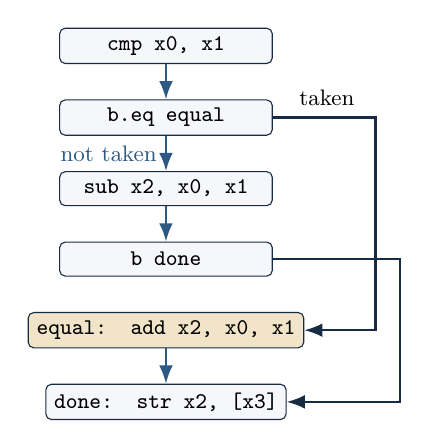
\begin{tikzpicture}[
  scale=.9,
  transform shape,
  node distance=.5cm,
  inst/.style={
    draw=navy,
    fill=softgray,
    rounded corners=2pt,
    minimum width=3.0cm,
    minimum height=.48cm,
    align=center,
    font=\small\ttfamily
  },
  note/.style={
    font=\small,
    align=center
  }
]

\node[inst] (i1) {cmp x0, x1};
\node[inst,below=of i1] (i2) {b.eq equal};
\node[inst,below=of i2] (i3) {sub x2, x0, x1};
\node[inst,below=of i3] (i4) {b done};
\node[inst,below=of i4,fill=gold!25] (i5) {equal: add x2, x0, x1};
\node[inst,below=of i5] (i6) {done: str x2, [x3]};

% Sequential flow
\draw[-{Latex},thick,deepblue]
  (i1.south) -- (i2.north);

\draw[-{Latex},thick,deepblue]
  (i2.south) --
  node[left,note]{not taken}
  (i3.north);

\draw[-{Latex},thick,deepblue]
  (i3.south) -- (i4.north);

\draw[-{Latex},thick,deepblue]
  (i5.south) -- (i6.north);

% Conditional branch to equal
\draw[-{Latex},thick,navy]
  (i2.east)
  -- ++(1.45,0)
  |- (i5.east);

\node[note, above right=0.05cm and 0.25cm of i2.east] {taken};

% Unconditional branch to done
\draw[-{Latex},thick,navy]
  (i4.east)
  -- ++(1.80,0)
  |- (i6.east);

\end{tikzpicture}
\end{center}

\vspace{-0.2cm}

\begin{block}{Branch Outcome}
A conditional branch either transfers control to its target or falls through to the next sequential instruction.
\end{block}
\end{frame}

% ============================================================
% Slide 7
% Slide Header: Comparisons and Condition Flags
% ============================================================
\sectiondivider{Section 02}{Comparisons and Condition Flags}

% ============================================================
% Slide 8
% Slide Header: cmp Updates Flags by Subtraction
% ============================================================
\begin{frame}{\code{cmp} Updates Flags by Subtraction}
\begin{block}{Underlying Operation}
\code{cmp x0, x1} performs a subtraction for flags and discards the numeric result.
\end{block}
\vspace{0.25cm}
\large
\hspace{3.8cm}\code{cmp x0, x1}\\[0.15cm]
\hspace{3.8cm}\code{subs xzr, x0, x1}
\normalsize
\vspace{0.25cm}
\begin{itemize}
\item The computed value \code{x0 - x1} is not kept as a data result.
\item NZCV is updated from the subtraction.
\item Later conditional branches inspect those flags.
\item This connects comparison directly to the flag-setting arithmetic from Topic 5.
\end{itemize}
\end{frame}

% ============================================================
% Slide 9
% Slide Header: The NZCV Flags Used by Branches
% ============================================================
\begin{frame}{The NZCV Flags Used by Branches}
\begin{center}

\begin{tikzpicture}[
  fld/.style={
    draw=navy,
    thick,
    minimum width=2.2cm,
    minimum height=1.0cm,
    align=center,
    font=\bfseries
  }
]
\node[fld,fill=navy,text=white] (n) {N\\Negative};
\node[fld,fill=deepblue,text=white,right=.15cm of n] (z) {Z\\Zero};
\node[fld,fill=gold!35,text=navy,right=.15cm of z] (c) {C\\Carry};
\node[fld,fill=softgray,text=navy,right=.15cm of c] (v) {V\\Overflow};
\end{tikzpicture}
\end{center}
\vspace{0.25cm}
\begin{itemize}
\item \key{Z}: equality after a compare.
\item \key{N} and \key{V}: signed ordering after subtraction.
\item \key{C}: unsigned ordering after subtraction; \code{C=1} means no unsigned borrow.
\item The same compare can support signed or unsigned branch decisions.
\end{itemize}
\end{frame}

% ============================================================
% Slide 10
% Slide Header: Equality Branches
% ============================================================
\begin{frame}{Equality Branches}
\begin{columns}[T,onlytextwidth]
\column{0.48\textwidth}
\begin{block}{Equal}
\large
\hspace{1.8cm}\code{b.eq target}
\normalsize
\begin{itemize}
\item Branches when \code{Z=1}.
\item Used after \code{cmp}, \code{subs}, or another flag-setting operation.
\end{itemize}
\end{block}
\column{0.48\textwidth}
\begin{block}{Not Equal}
\large
\hspace{1.7cm}\code{b.ne target}
\normalsize
\begin{itemize}
\item Branches when \code{Z=0}.
\item Common for loop continuation and mismatch tests.
\end{itemize}
\end{block}
\end{columns}
\vspace{0.25cm}
\begin{block}{Example}
\large
\hspace{3.3cm}\code{cmp x0, x1}\\[0.12cm]
\hspace{3.3cm}\code{b.eq equal\_case}
\normalsize
\end{block}
\end{frame}

% ============================================================
% Slide 11
% Slide Header: Signed and Unsigned Ordering
% ============================================================
\begin{frame}{Signed and Unsigned Ordering}
\begin{center}
\small
\renewcommand{\arraystretch}{1.15}
\begin{tabular}{
  >{\raggedright\arraybackslash}m{2.7cm}
  >{\raggedright\arraybackslash}m{3.8cm}
  >{\raggedright\arraybackslash}m{4.7cm}
}
\rowcolor{navy}
{\color{white}\bfseries Branch} &
{\color{white}\bfseries Interpretation} &
{\color{white}\bfseries Condition after \code{cmp x0, x1}} \\
\rowcolor{softgray}
\code{b.lt label} &
signed less than &
\code{x0 < x1} as two's complement, $N \ne V$ \\
\rowcolor{white}
\code{b.ge label} &
signed greater/equal &
\code{x0 >= x1} as two's complement, $N = V$ \\
\rowcolor{softgray}
\code{b.lo label} &
unsigned lower &
\code{x0 < x1} as unsigned, $C=0$ \\
\rowcolor{white}
\code{b.hs label} &
unsigned higher/same &
\code{x0 >= x1} as unsigned, $C=1$ \\
\end{tabular}
\end{center}
\vspace{0.25cm}
\begin{block}{Important Distinction}
Do not use signed and unsigned branch mnemonics interchangeably. They inspect different flag evidence.
\end{block}
\end{frame}

% ============================================================
% Slide 12
% Slide Header: Same cmp, Different Meaning
% ============================================================
\begin{frame}{Same \code{cmp}, Different Meaning}
\begin{block}{Example Bit Patterns}
For 8-bit intuition, compare \code{0xff} with \code{0x01}. The bit patterns are the same, but the numerical interpretation changes.
\end{block}
\vspace{0.15cm}
\begin{center}
\small
\renewcommand{\arraystretch}{1.18}
\begin{tabular}{
  >{\raggedright\arraybackslash}m{3.2cm}
  >{\raggedright\arraybackslash}m{3.5cm}
  >{\raggedright\arraybackslash}m{4.2cm}
}
\rowcolor{navy}
{\color{white}\bfseries Interpretation} &
{\color{white}\bfseries Values} &
{\color{white}\bfseries Correct ordering} \\
\rowcolor{softgray}
Unsigned & $255$ and $1$ & $255 > 1$ \\
\rowcolor{white}
Signed two's complement & $-1$ and $1$ & $-1 < 1$ \\
\end{tabular}
\end{center}
\vspace{0.25cm}
\begin{block}{AArch64 Consequence}
After the same comparison, \code{b.lo} and \code{b.lt} may lead to different control-flow paths.
\end{block}
\end{frame}

% ============================================================
% Slide 13
% Slide Header: Branch Instructions
% ============================================================
\sectiondivider{Section 03}{Branch Instructions}

% ============================================================
% Slide 14
% Slide Header: Unconditional Branch
% ============================================================
\begin{frame}{Unconditional Branch}
\begin{block}{Branch Always}
\code{b label} transfers control to the target label without testing NZCV flags.
\end{block}
\vspace{0.25cm}
\large
\hspace{4.0cm}\code{b done}\\[0.15cm]
\hspace{4.0cm}\code{add x0, x0, \#1}\\[0.15cm]
\hspace{4.0cm}\code{done:}
\normalsize
\vspace{0.25cm}
\begin{itemize}
\item Used to skip over an alternative block.
\item Used at the bottom of loops to return to the loop test or loop body.
\item Does not depend on signed or unsigned interpretation.
\end{itemize}
\end{frame}

% ============================================================
% Slide 15
% Slide Header: Conditional Branch Pattern
% ============================================================
\begin{frame}{Conditional Branch Pattern}
\begin{block}{Two-Step Decision}
A common AArch64 decision first sets flags, then uses a branch instruction to test those flags.
\end{block}
\vspace{0.2cm}
\begin{columns}[T,onlytextwidth]
\column{0.48\textwidth}
\begin{block}{Step 1: Compare}
\large
\hspace{1.7cm}\code{cmp x0, x1}
\normalsize
\begin{itemize}
\item Computes \code{x0 - x1} for flags.
\item Updates NZCV.
\item Does not keep the subtraction result.
\end{itemize}
\end{block}
\column{0.48\textwidth}
\begin{block}{Step 2: Branch}
\large
\hspace{1.5cm}\code{b.lt less}
\normalsize
\begin{itemize}
\item Tests the relevant flag condition.
\item Redirects control if the condition is true.
\item Falls through otherwise.
\end{itemize}
\end{block}
\end{columns}
\end{frame}

% ============================================================
% Slide 16
% Slide Header: Common Conditional Branch Mnemonics
% ============================================================
\begin{frame}{Common Conditional Branch Mnemonics}
\begin{center}
\small
\renewcommand{\arraystretch}{1.12}
\begin{tabular}{
  >{\raggedright\arraybackslash}m{2.0cm}
  >{\raggedright\arraybackslash}m{3.0cm}
  >{\raggedright\arraybackslash}m{2.0cm}
  >{\raggedright\arraybackslash}m{3.3cm}
}
\rowcolor{navy}
{\color{white}\bfseries Branch} &
{\color{white}\bfseries Meaning} &
{\color{white}\bfseries Branch} &
{\color{white}\bfseries Meaning} \\
\rowcolor{softgray}
\code{b.eq} & equal &
\code{b.ne} & not equal \\
\rowcolor{white}
\code{b.lt} & signed less than &
\code{b.ge} & signed greater/equal \\
\rowcolor{softgray}
\code{b.gt} & signed greater than &
\code{b.le} & signed less/equal \\
\rowcolor{white}
\code{b.lo} & unsigned lower &
\code{b.hs} & unsigned higher/same \\
\rowcolor{softgray}
\code{b.hi} & unsigned higher &
\code{b.ls} & unsigned lower/same \\
\end{tabular}
\end{center}
\vspace{0.2cm}
\begin{block}{Mnemonic Choice}
The comparison operation may be identical, but the branch mnemonic determines how the flags are interpreted.
\end{block}
\end{frame}

% ============================================================
% Slide 17
% Slide Header: Compare and Branch on Zero
% ============================================================
\begin{frame}{Compare and Branch on Zero}
\begin{columns}[T,onlytextwidth]
\column{0.48\textwidth}
\begin{block}{Branch if Zero}
\large
\hspace{1.5cm}\code{cbz x0, target}
\normalsize
\begin{itemize}
\item Tests whether \code{x0} equals zero.
\item Branches if the test is true.
\item Does not update NZCV flags.
\end{itemize}
\end{block}
\column{0.48\textwidth}
\begin{block}{Branch if Nonzero}
\large
\hspace{1.4cm}\code{cbnz x0, target}
\normalsize
\begin{itemize}
\item Tests whether \code{x0} is nonzero.
\item Branches if the test is true.
\item Useful for pointer and counter tests.
\end{itemize}
\end{block}
\end{columns}
\vspace{0.25cm}
\begin{block}{No Flag Side Effect}
These instructions test a register directly. Existing NZCV values are left unchanged.
\end{block}
\end{frame}

% ============================================================
% Slide 18
% Slide Header: Test Bit and Branch
% ============================================================
\begin{frame}{Test Bit and Branch}
\begin{block}{Bit-Specific Control Flow}
\code{tbz} and \code{tbnz} test a selected bit and branch according to whether that bit is zero or nonzero.
\end{block}
\vspace{0.2cm}
\begin{columns}[T,onlytextwidth]
\column{0.48\textwidth}
\begin{block}{Test Bit Zero}
\large
\hspace{1.1cm}\code{tbz x0, \#3, clear}
\normalsize
\begin{itemize}
\item Tests bit 3 of \code{x0}.
\item Branches if the bit is 0.
\item Does not update NZCV.
\end{itemize}
\end{block}
\column{0.48\textwidth}
\begin{block}{Test Bit Nonzero}
\large
\hspace{1.0cm}\code{tbnz x0, \#3, set}
\normalsize
\begin{itemize}
\item Tests bit 3 of \code{x0}.
\item Branches if the bit is 1.
\item Does not update NZCV.
\end{itemize}
\end{block}
\end{columns}
\end{frame}

% ============================================================
% Slide 19
% Slide Header: Branches and Flags
% ============================================================
\begin{frame}{Branches and Flags}
\begin{center}
\small
\renewcommand{\arraystretch}{1.16}
\begin{tabular}{
  >{\raggedright\arraybackslash}m{3.0cm}
  >{\raggedright\arraybackslash}m{4.0cm}
  >{\raggedright\arraybackslash}m{4.2cm}
}
\rowcolor{navy}
{\color{white}\bfseries Branch form} &
{\color{white}\bfseries Tests} &
{\color{white}\bfseries NZCV effect} \\
\rowcolor{softgray}
\code{b.cond label} &
Existing condition flags &
Reads NZCV; does not update it \\
\rowcolor{white}
\code{cbz/cbnz} &
Register equals zero or nonzero &
Does not update NZCV \\
\rowcolor{softgray}
\code{tbz/tbnz} &
One selected register bit &
Does not update NZCV \\
\rowcolor{white}
\code{b label} &
No condition &
Does not test or update NZCV \\
\end{tabular}
\end{center}
\vspace{0.25cm}
\begin{block}{Programming Implication}
Use \code{b.cond} when NZCV already contains the needed comparison. Use a direct-test branch when the decision depends only on zero, nonzero, or one selected bit.
\end{block}
\end{frame}

% ============================================================
% Slide 20
% Slide Header: Selection Structures
% ============================================================
\sectiondivider{Section 04}{Selection Structures}

% ============================================================
% Slide 21
% Slide Header: Translating an if Statement
% ============================================================
\begin{frame}{Translating an \code{if} Statement}
\begin{columns}[T,onlytextwidth]
\column{0.43\textwidth}
\begin{block}{C}
\large
\hspace{0.6cm}\code{if (x == y) \{}\\[0.10cm]
\hspace{1.1cm}\code{z = x + y;}\\[0.10cm]
\hspace{0.6cm}\code{\}}
\normalsize
\end{block}
\column{0.53\textwidth}
\begin{block}{AArch64}
\large
\hspace{0.7cm}\code{cmp x0, x1}\\[0.10cm]
\hspace{0.7cm}\code{b.ne endif}\\[0.10cm]
\hspace{0.7cm}\code{add x2, x0, x1}\\[0.10cm]
\hspace{0.7cm}\code{endif:}
\normalsize
\end{block}
\end{columns}
\vspace{0.2cm}
\begin{block}{Control-Flow Shape}
The branch often tests the opposite of the high-level condition so execution can skip the body when the condition is false.
\end{block}
\end{frame}

% ============================================================
% Slide 22
% Slide Header: Translating if-else
% ============================================================
\begin{frame}{Translating \code{if}-\code{else}}
\begin{columns}[T,onlytextwidth]
\column{0.43\textwidth}
\begin{block}{C}
\small
\hspace{0.4cm}\code{if (x == y) \{}\\[0.08cm]
\hspace{0.8cm}\code{z = x + y;}\\[0.08cm]
\hspace{0.4cm}\code{\} else \{}\\[0.08cm]
\hspace{0.8cm}\code{z = x - y;}\\[0.08cm]
\hspace{0.4cm}\code{\}}
\end{block}
\column{0.53\textwidth}
\begin{block}{AArch64}
\small
\hspace{0.7cm}\code{cmp x0, x1}\\[0.08cm]
\hspace{0.7cm}\code{b.ne else\_case}\\[0.08cm]
\hspace{0.7cm}\code{add x2, x0, x1}\\[0.08cm]
\hspace{0.7cm}\code{b end\_if}\\[0.08cm]
\hspace{0.7cm}\code{else\_case:}\\[0.08cm]
\hspace{0.7cm}\code{sub x2, x0, x1}\\[0.08cm]
\hspace{0.7cm}\code{end\_if:}
\end{block}
\end{columns}
\vspace{0.15cm}
\begin{block}{Unconditional Skip}
The unconditional branch after the true block prevents fall-through into the false block.
\end{block}
\end{frame}

% ============================================================
% Slide 23
% Slide Header: Loops and Applied Traversal
% ============================================================
\sectiondivider{Section 05}{Loops and Applied Traversal}

% ============================================================
% Slide 24
% Slide Header: Translating a while Loop
% ============================================================
\begin{frame}{Translating a \code{while} Loop}
\begin{columns}[T,onlytextwidth]
\column{0.43\textwidth}
\begin{block}{C}
\small
\hspace{0.4cm}\code{while (i < n) \{}\\[0.08cm]
\hspace{0.8cm}\code{sum += a[i];}\\[0.08cm]
\hspace{0.8cm}\code{i++;}\\[0.08cm]
\hspace{0.4cm}\code{\}}
\end{block}
\column{0.53\textwidth}
\begin{block}{AArch64 Skeleton}
\small
\hspace{0.5cm}\code{loop\_test:}\\[0.08cm]
\hspace{0.5cm}\code{cmp x1, x2}\\[0.08cm]
\hspace{0.5cm}\code{b.ge loop\_done}\\[0.08cm]
\hspace{0.5cm}\code{// loop body}\\[0.08cm]
\hspace{0.5cm}\code{add x1, x1, \#1}\\[0.08cm]
\hspace{0.5cm}\code{b loop\_test}\\[0.08cm]
\hspace{0.5cm}\code{loop\_done:}
\end{block}
\end{columns}
\vspace{0.15cm}
\begin{block}{Test Before Body}
A \code{while} loop checks its condition before executing the body, so the body may execute zero times.
\end{block}
\end{frame}

% ============================================================
% Slide 25
% Slide Header: Translating a do-while Loop
% ============================================================
\begin{frame}{Translating a \code{do}-\code{while} Loop}
\begin{columns}[T,onlytextwidth]
\column{0.43\textwidth}
\begin{block}{C}
\small
\hspace{0.4cm}\code{do \{}\\[0.08cm]
\hspace{0.8cm}\code{x += step;}\\[0.08cm]
\hspace{0.4cm}\code{\} while (x < limit);}
\end{block}
\column{0.53\textwidth}
\begin{block}{AArch64}
\small
\hspace{0.5cm}\code{loop\_body:}\\[0.08cm]
\hspace{0.5cm}\code{add x0, x0, x1}\\[0.08cm]
\hspace{0.5cm}\code{cmp x0, x2}\\[0.08cm]
\hspace{0.5cm}\code{b.lt loop\_body}
\end{block}
\end{columns}
\vspace{0.15cm}
\begin{block}{Test After Body}
A \code{do}-\code{while} loop executes the body once before its first condition test. Here, \code{x0}, \code{x1}, and \code{x2} represent \code{x}, \code{step}, and \code{limit}.
\end{block}
\end{frame}

% ============================================================
% Slide 26
% Slide Header: Counted Loop with subs
% ============================================================
\begin{frame}{Counted Loop with \code{subs}}
\begin{block}{Decrement and Test}
A decrementing loop can combine counter update and flag update using \code{subs}.
\end{block}
\vspace{0.25cm}
\large
\hspace{3.6cm}\code{loop:}\\[0.12cm]
\hspace{3.6cm}\code{// loop body}\\[0.12cm]
\hspace{3.6cm}\code{subs x0, x0, \#1}\\[0.12cm]
\hspace{3.6cm}\code{b.ne loop}
\normalsize
\vspace{0.25cm}
\begin{itemize}
\item \code{subs} decrements \code{x0} and updates NZCV.
\item \code{b.ne} repeats while the result is not zero.
\item This works naturally when the initial count is positive.
\end{itemize}
\end{frame}

% ============================================================
% Slide 27
% Slide Header: Array Traversal Loop
% ============================================================
\begin{frame}{Array Traversal Loop}
\begin{block}{Example}
Sum \code{n} 64-bit integers. Let \code{x0} hold the base pointer, \code{x1} hold \code{n}, and \code{x2} hold the running sum.
\end{block}
\vspace{0.05cm}
\small
\hspace{2.8cm}\code{mov x2, xzr}\\[0.05cm]
\hspace{2.8cm}\code{loop:}\\[0.05cm]
\hspace{2.8cm}\code{cbz x1, done}\\[0.05cm]
\hspace{2.8cm}\code{ldr x3, [x0], \#8}\\[0.05cm]
\hspace{2.8cm}\code{add x2, x2, x3}\\[0.05cm]
\hspace{2.8cm}\code{sub x1, x1, \#1}\\[0.05cm]
\hspace{2.8cm}\code{b loop}\\[0.05cm]
\hspace{2.8cm}\code{done:}
\vspace{0.05cm}
\begin{block}{Pointer Update}
\code{ldr x3, [x0], \#8} loads the current element and advances the pointer by one 64-bit element.
\end{block}
\end{frame}

% ============================================================
% Slide 28
% Slide Header: String Traversal Loop
% ============================================================
\begin{frame}{String Traversal Loop}
\begin{block}{Null-Terminated Strings}
A C string ends with a zero byte. Byte loads are used so the loop tests one character at a time.
\end{block}
\vspace{0.15cm}
\small
\hspace{3.0cm}\code{loop:}\\[0.08cm]
\hspace{3.0cm}\code{ldrb w1, [x0], \#1}\\[0.08cm]
\hspace{3.0cm}\code{cbz w1, done}\\[0.08cm]
\hspace{3.0cm}\code{// process character in w1}\\[0.08cm]
\hspace{3.0cm}\code{b loop}\\[0.08cm]
\hspace{3.0cm}\code{done:}
\vspace{0.15cm}
\begin{itemize}
\item \code{ldrb} reads one byte and zero-extends into \code{w1}.
\item Post-indexing advances \code{x0} after the load.
\item \code{cbz} tests for the null terminator without modifying NZCV.
\end{itemize}
\end{frame}

% ============================================================
% Slide 29
% Slide Header: Common Branching Mistakes
% ============================================================
\begin{frame}{Common Branching Mistakes}
\begin{itemize}
\item Using \code{b.lt} for an unsigned comparison that should use \code{b.lo}.
\item Forgetting that \code{cmp x0, x1} means the flags reflect \code{x0 - x1}, not \code{x1 - x0}.
\item Assuming \code{cbz}, \code{cbnz}, \code{tbz}, or \code{tbnz} update NZCV flags.
\item Omitting the unconditional branch needed to skip an \code{else} block.
\item Placing a loop update after a branch target where it no longer executes on every iteration.
\end{itemize}
\vspace{0.15cm}
\begin{block}{Debugging Practice}
Trace the values, then trace the flags, then trace the branch target. Avoid guessing from the high-level source alone.
\end{block}
\end{frame}

% ============================================================
% Slide 30
% Slide Header: Summary and Self-Test
% ============================================================
\sectiondivider{Section 06}{Summary and Self-Test}

% ============================================================
% Slide 31
% Slide Header: Topic 7 Summary
% ============================================================
\begin{frame}{Topic 7 Summary}
\begin{itemize}
\item The program counter determines the current control-flow position, but it is not an ordinary AArch64 general-purpose register.
\item \code{cmp} updates NZCV by performing a flag-setting subtraction and discarding the result.
\item Conditional branches use flags, while \code{cbz}, \code{cbnz}, \code{tbz}, and \code{tbnz} test registers directly without updating NZCV.
\item Signed and unsigned branch mnemonics must be selected according to the intended interpretation.
\item High-level \code{if}, \code{else}, \code{while}, and \code{do}-\code{while} constructs translate into labels, comparisons, conditional branches, and fall-through paths.
\end{itemize}
\end{frame}

% ============================================================
% Slide 32
% Slide Header: Self-Test 1/2
% ============================================================
\begin{frame}{Self-Test 1/2}
\begin{enumerate}
\item What does \code{cmp x0, x1} compute internally, and where is the result stored?
\item Why can the same \code{cmp} support both signed and unsigned comparisons?
\item Which branch should be used for unsigned lower-than: \code{b.lt} or \code{b.lo}?
\item What does \code{b.eq} test after a comparison?
\item Why is an unconditional \code{b} often needed in an \code{if}-\code{else} translation?
\end{enumerate}
\end{frame}

% ============================================================
% Slide 33
% Slide Header: Self-Test 2/2
% ============================================================
\begin{frame}{Self-Test 2/2}
\begin{enumerate}
\setcounter{enumi}{5}
\item How does \code{cbz x0, target} differ from \code{cmp x0, xzr} followed by \code{b.eq target}?
\item Why does \code{ldrb w1, [x0], \#1} help with string traversal?
\item What is the difference between a \code{while} loop and a \code{do}-\code{while} loop in branch structure?
\item How do \code{tbz} and \code{tbnz} differ from flag-based conditional branches?
\item Why must a loop update execute before control branches back to the next test?
\end{enumerate}
\end{frame}

% ============================================================
% Slide 34
% Slide Header: Review Exercise
% ============================================================
\begin{frame}{Review Exercise}
\begin{block}{Classify the Branch Behavior}
For each instruction, state whether it reads NZCV, updates NZCV, directly tests a register, or branches unconditionally.
\end{block}
\vspace{0.15cm}
\begin{center}
\small
\renewcommand{\arraystretch}{1.16}
\begin{tabular}{
  >{\raggedright\arraybackslash}m{4.2cm}
  >{\raggedright\arraybackslash}m{6.3cm}
}
\rowcolor{navy}
{\color{white}\bfseries Instruction} &
{\color{white}\bfseries Classification} \\
\rowcolor{softgray}
\code{b.eq target} & \\
\rowcolor{white}
\code{cbz x0, target} & \\
\rowcolor{softgray}
\code{tbz x1, \#4, target} & \\
\rowcolor{white}
\code{b target} & \\
\rowcolor{softgray}
\code{cmp x0, x1} & \\
\end{tabular}
\end{center}
\end{frame}

% ============================================================
% Slide 35
% Slide Header: Next Topic
% ============================================================
\begin{frame}{Next Topic}
\begin{block}{Procedures and the Stack}
Topic 8 develops the conventions and memory organization needed for reliable procedure calls.
\end{block}
\vspace{0.25cm}
\begin{itemize}
\item Procedure calls and returns
\item Stack organization
\item Parameter passing
\item Calling conventions
\end{itemize}
\end{frame}

\end{document}